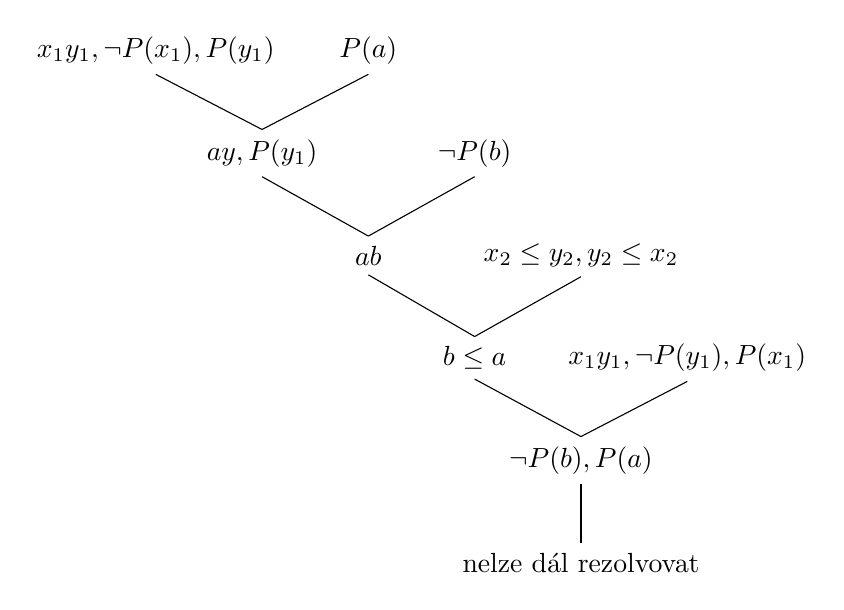
\begin{tikzpicture}[
grow'=up,
note/.style={font=\footnotesize,black!65},
level/.style={sibling distance=2.7cm},
level distance =1.3cm,
parent anchor=north,
child anchor=south]
\node {nelze dál rezolvovat}
    child {node {$ \neg P(b), P(a) $}
        child {node {$ b\leq a $}
            child {node {$ a\nleq b $}
                child {node {$ a\nleq y, P(y_1) $}
                    child {node {$ x_1\nleq y_1, \neg P(x_1), P(y_1) $}}
                    child {node {$ P(a) $}}}
                child {node {$ \neg P(b) $}}}
            child {node {$ x_2\leq y_2, y_2\leq x_2 $}}}
        child {node {$ x_1\nleq y_1,\neg P(y_1),P(x_1) $}}};
\end{tikzpicture}